\documentclass[tikz,border=12pt]{standalone}
\usepackage[T1]{fontenc}
\usepackage{helvet}
\renewcommand{\familydefault}{\sfdefault}
\usepackage{amsmath}
\usetikzlibrary{arrows.meta, fit, backgrounds, positioning, calc, shapes.geometric}

% Semantic palette, shared across the method figures. Color encodes role:
%   blue   = BM25 / lexical step
%   red    = LLM step
%   amber  = document data and stores
%   green  = retrieved units and final output (leaves, candidates, passages)
%   gray   = query input
\definecolor{queryfill}{HTML}{ECEFF2}   % gray, input
\definecolor{queryborder}{HTML}{8A96A3}
\definecolor{bm25fill}{HTML}{E2ECF7}     % blue, BM25 step
\definecolor{bm25border}{HTML}{3C6CA6}
\definecolor{llmfill}{HTML}{F7E4E4}      % red, LLM step
\definecolor{llmborder}{HTML}{BE4F4F}
\definecolor{corpusfill}{HTML}{FBF0D5}   % amber, document data and stores
\definecolor{corpusborder}{HTML}{CFA23E}
\definecolor{outfill}{HTML}{E7F4E7}      % green, retrieved units and output
\definecolor{outborder}{HTML}{59A05B}
\definecolor{poolfill}{HTML}{F1F9F1}
\definecolor{regfill}{HTML}{F6F8FB}
\definecolor{regborder}{HTML}{C4CDD6}
\definecolor{darkline}{HTML}{333333}
\definecolor{subtext}{HTML}{5A5A5A}

\tikzset{
  card/.style={rectangle, rounded corners=5pt, align=center, draw=darkline,
               line width=0.8pt, minimum height=1.2cm, font=\small},
  query/.style={card, fill=queryfill, draw=queryborder, minimum width=2.0cm},
  proc/.style={card, fill=bm25fill, draw=bm25border, minimum width=2.7cm},
  llmproc/.style={card, fill=llmfill, draw=llmborder, minimum width=2.7cm},
  result/.style={card, fill=outfill, draw=outborder, minimum width=2.2cm},
  leaf/.style={rectangle, rounded corners=3pt, draw=outborder, fill=outfill,
               line width=0.8pt, minimum width=1.05cm, minimum height=0.82cm, font=\scriptsize},
  db/.style={cylinder, shape border rotate=90, aspect=0.28, draw=corpusborder,
             fill=corpusfill, line width=0.8pt, minimum width=1.75cm,
             minimum height=1.05cm, font=\scriptsize, align=center, inner sep=1pt},
  region/.style={rounded corners=12pt, fill=regfill, draw=regborder, line width=0.8pt},
  pooldash/.style={draw=outborder, dashed, rounded corners=8pt, fill=poolfill,
                   line width=0.85pt},
  regtitle/.style={font=\small\bfseries, text=darkline},
  note/.style={font=\scriptsize\itshape, text=subtext, align=center},
  flow/.style={-{Latex[length=2.2mm]}, line width=0.85pt, draw=darkline},
  feed/.style={-{Latex[length=1.9mm]}, line width=0.7pt, draw=corpusborder},
}

\def\inlen{0.9cm}
\def\stagegap{1.7cm}
\def\intra{1.0cm}
\def\lspread{1.25cm}
\def\cspread{1.0cm}
\def\dbdrop{1.0cm}

\begin{document}
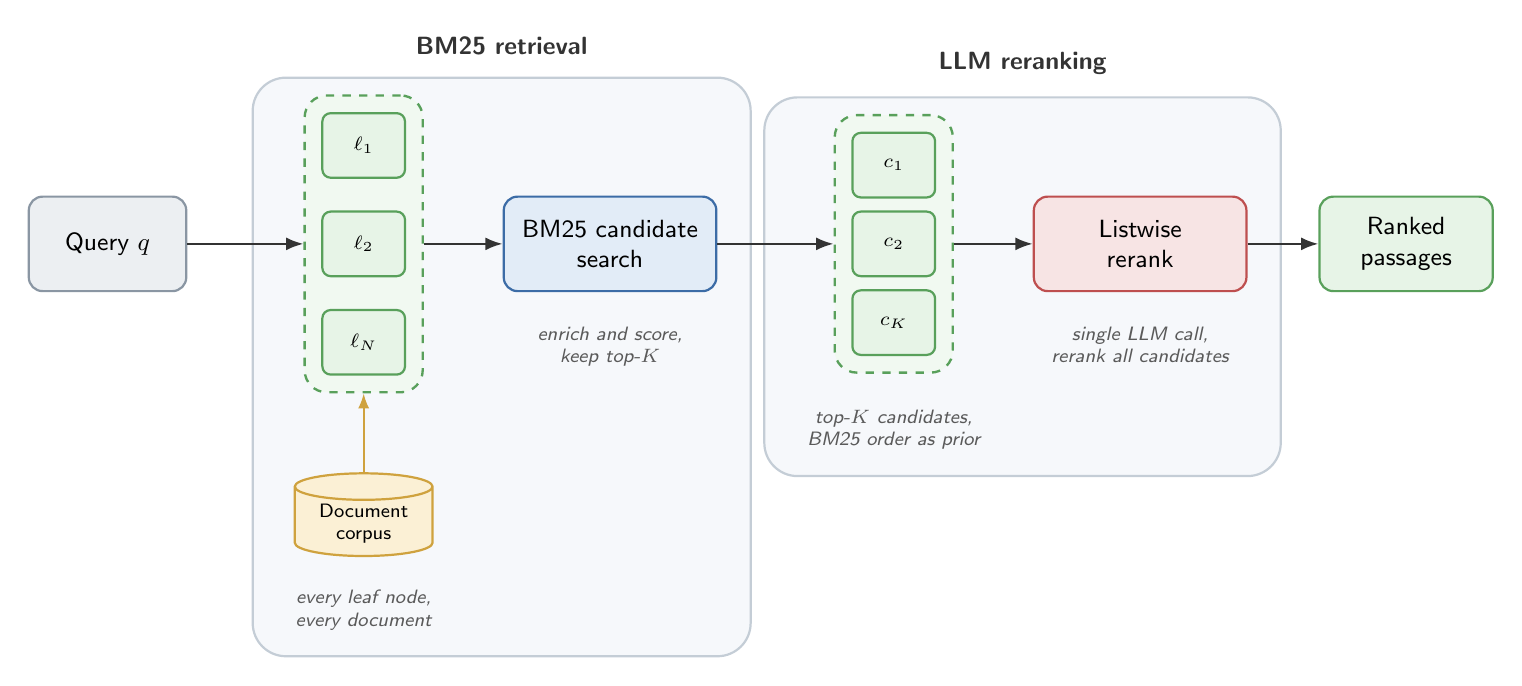
\begin{tikzpicture}

% Input (outside the phases)
\node[query] (query) {Query $q$};

% Stage 1: BM25 retrieval over the flat corpus
\node[leaf, right=\stagegap of query, yshift=\lspread]  (lf1) {$\ell_1$};
\node[leaf, right=\stagegap of query]                   (lf2) {$\ell_2$};
\node[leaf, right=\stagegap of query, yshift=-\lspread] (lfn) {$\ell_N$};
\node[font=\footnotesize] at ($(lf2)!0.5!(lfn)$) {$\vdots$};
\node[pooldash, fit=(lf1)(lf2)(lfn), inner sep=6pt] (pool) {};
\foreach \n/\t in {lf1/\ell_1, lf2/\ell_2, lfn/\ell_N} {
  \node[leaf] at (\n) {$\t$};
}
\node[db, below=\dbdrop of pool] (corpus) {Document\\corpus};
\node[proc, right=\intra of pool] (bm25) {BM25 candidate\\search};

% Stage 2: LLM listwise rerank of the top-K candidates, in BM25 order
\node[leaf, right=\stagegap of bm25, yshift=\cspread]  (c1) {$c_1$};
\node[leaf, right=\stagegap of bm25]                   (c2) {$c_2$};
\node[leaf, right=\stagegap of bm25, yshift=-\cspread] (ck) {$c_K$};
\node[font=\footnotesize] at ($(c2)!0.5!(ck)$) {$\vdots$};
\node[pooldash, fit=(c1)(c2)(ck), inner sep=6pt] (cpool) {};
\foreach \n/\t in {c1/c_1, c2/c_2, ck/c_K} {
  \node[leaf] at (\n) {$\t$};
}
\node[llmproc, right=\intra of cpool] (llm) {Listwise\\rerank};

% Output (outside the phases)
\node[result, right=\inlen of llm] (sources) {Ranked\\passages};

% Notes
\node[note, below=0.30cm of corpus] (corpusnote) {every leaf node,\\every document};
\node[note, below=0.32cm of bm25] (bm25note) {enrich and score,\\keep top-$K$};
\node[note, below=0.34cm of cpool] (candnote) {top-$K$ candidates,\\BM25 order as prior};
\node[note, below=0.32cm of llm] (llmnote) {single LLM call,\\rerank all candidates};

% Phase panels. Input and output stay outside.
\begin{scope}[on background layer]
  \coordinate (bandB) at ($(corpus.south)+(0,-0.14)$);
  \node[region, inner xsep=12pt, inner ysep=6pt,
        fit=(pool)(corpus)(corpusnote)(bm25)(bm25note)(pool|-bandB)] (reg1) {};
  \node[region, inner xsep=12pt, inner ysep=6pt,
        fit=(cpool)(candnote)(llm)(llmnote)] (reg2) {};
\end{scope}
\node[regtitle, anchor=south] at ($(reg1.north)+(0,0.16)$) {BM25 retrieval};
\node[regtitle, anchor=south] at ($(reg2.north)+(0,0.16)$) {LLM reranking};

% Flow
\draw[flow] (query) -- (pool.west);
\draw[feed] (corpus.north) -- (pool.south);
\draw[flow] (pool.east) -- (bm25.west);
\draw[flow] (bm25.east) -- (cpool.west);
\draw[flow] (cpool.east) -- (llm.west);
\draw[flow] (llm.east) -- (sources.west);

\end{tikzpicture}
\end{document}
